\documentclass{article}
\usepackage[paperwidth=7.16in, paperheight=7.6in, margin=0in]{geometry}

\usepackage{tikz}
\usetikzlibrary{positioning}
\usetikzlibrary{positioning, external}
\tikzset{external/system call={pdflatex \tikzexternalcheckshellescape -halt-on-error 
-interaction=batchmode -jobname "\image" "\texsource" && % or ;
pdftops -eps "\image".pdf}}
\tikzexternalize

\begin{document}
% \tikzstyle{boundline} = [draw, line width=.5, black]
% \tikzstyle{courtline} = [draw, line width=.5, black]
% \tikzstyle{textcolor} = [black]
% \tikzstyle{markercolor} = [black]

\tikzstyle{cell} = [rectangle, outer sep=0pt, inner sep = 0]

\def\innersep{0.05in}
\def\scl{1.1in}
\def\sclBig{2.2in}
\def\labelShift{-2.8cm}

\begin{tikzpicture}[node distance=0pt]
	\begin{scope}

		\node[cell]	(S_A_BEST) at (0, 0)	{\includegraphics[width=\sclBig]{../data/Courts/SynthA/Result_best.png}};
		\node[cell, left = of S_A_BEST, anchor=south east]	(S_A_START)	{\includegraphics[width=\scl]{../data/Courts/SynthA/Result_start.png}};
		\node[cell, below = of S_A_START]	(S_A_FITNESS)	{\includegraphics[width=\scl]{../data/Courts/SynthA/Result_fitness.png}};
		\node[cell, above right = 0in and \innersep of S_A_BEST, anchor=north west]	(S_B_START)	{\includegraphics[width=\scl]{../data/Courts/SynthB/Result_start.png}};
		\node[cell, below = of S_B_START]	(S_B_FITNESS)	{\includegraphics[width=\scl]{../data/Courts/SynthB/Result_fitness.png}};
		\node[cell, above right = of S_B_START, anchor=north west]	(S_B_BEST)	{\includegraphics[width=\sclBig]{../data/Courts/SynthB/Result_best.png}};

		\node[below = of S_A_BEST, align=center]	(S_A_LABEL) {\hspace{\labelShift}(a)};
		\node[below = of S_B_BEST, align=center]	(S_B_LABEL) {\hspace{\labelShift}(b)};

		\node[cell, below = of S_A_LABEL, anchor=north]	(S_C_BEST)	{\includegraphics[width=\sclBig]{../data/Courts/SynthC/Result_best.png}};
		\node[cell, left = of S_C_BEST, anchor=south east]	(S_C_START)	{\includegraphics[width=\scl]{../data/Courts/SynthC/Result_start.png}};
		\node[cell, below = of S_C_START]	(S_C_FITNESS)	{\includegraphics[width=\scl]{../data/Courts/SynthC/Result_fitness.png}};
		\node[cell, above right = 0in and \innersep  of S_C_BEST, anchor=north west]	(S_D_START)	{\includegraphics[width=\scl]{../data/Courts/SynthD/Result_start.png}};
		\node[cell, below = of S_D_START]	(S_D_FITNESS)	{\includegraphics[width=\scl]{../data/Courts/SynthD/Result_fitness.png}};
		\node[cell, above right = of S_D_START, anchor=north west]	(S_D_BEST)	{\includegraphics[width=\sclBig]{../data/Courts/SynthD/Result_best.png}};

		\node[below = of S_C_BEST, align=center]	(S_C_LABEL) {\hspace{\labelShift}(c)};
		\node[below = of S_D_BEST, align=center]	(S_D_LABEL) {\hspace{\labelShift}(d)};

		\node[cell, below = of S_C_LABEL, anchor=north]	(C_A_BEST)	{\includegraphics[width=\sclBig]{../data/Courts/CourtA/Result_best.png}};
		\node[cell, left = of C_A_BEST, anchor=south east]	(C_A_START)	{\includegraphics[width=\scl]{../data/Courts/CourtA/Result_start.png}};
		\node[cell, below = of C_A_START]	(C_A_FITNESS)	{\includegraphics[width=\scl]{../data/Courts/CourtA/Result_fitness.png}};
		\node[cell, above right = 0in and \innersep  of C_A_BEST, anchor=north west]	(C_B_START)	{\includegraphics[width=\scl]{../data/Courts/CourtC/Result_start.png}};
		\node[cell, below = of C_B_START]	(C_B_FITNESS)	{\includegraphics[width=\scl]{../data/Courts/CourtC/Result_fitness.png}};
		\node[cell, above right = of C_B_START, anchor=north west]	(C_B_BEST)	{\includegraphics[width=\sclBig]{../data/Courts/CourtC/Result_best.png}};

		\node[below = of C_A_BEST, align=center]	(C_A_LABEL) {\hspace{\labelShift}(e)};
		\node[below = of C_B_BEST, align=center]	(C_B_LABEL) {\hspace{\labelShift}(f)};

		\node[cell, below = of C_A_LABEL, anchor=north]	(C_C_BEST)	{\includegraphics[width=\sclBig]{../data/Courts/CourtB/Result_best.png}};
		\node[cell, left = of C_C_BEST, anchor=south east]	(C_C_START)	{\includegraphics[width=\scl]{../data/Courts/CourtB/Result_start.png}};
		\node[cell, below = of C_C_START]	(C_C_FITNESS)	{\includegraphics[width=\scl]{../data/Courts/CourtB/Result_fitness.png}};
		\node[cell, above right = 0in and \innersep  of C_C_BEST, anchor=north west]	(C_D_START)	{\includegraphics[width=\scl]{../data/Courts/CourtD/Result_start.png}};
		\node[cell, below = of C_D_START]	(C_D_FITNESS)	{\includegraphics[width=\scl]{../data/Courts/CourtD/Result_fitness.png}};
		\node[cell, above right = of C_D_START, anchor=north west]	(C_D_BEST)	{\includegraphics[width=\sclBig]{../data/Courts/CourtD/Result_best.png}};

		\node[below = of C_C_BEST, align=center]	(C_C_LABEL) {\hspace{\labelShift}(g)};
		\node[below = of C_D_BEST, align=center]	(C_D_LABEL) {\hspace{\labelShift}(h)};


		\node[cell, below = of C_C_LABEL, anchor=north]	(C_E_BEST)	{\includegraphics[width=\sclBig]{../data/Courts/CourtE/Result_best.png}};
		\node[cell, left = of C_E_BEST, anchor=south east]	(C_E_START)	{\includegraphics[width=\scl]{../data/Courts/CourtE/Result_start.png}};
		\node[cell, below = of C_E_START]	(C_E_FITNESS)	{\includegraphics[width=\scl]{../data/Courts/CourtE/Result_fitness.png}};
		\node[cell, above right = 0in and \innersep  of C_E_BEST, anchor=north west]	(C_F_START)	{\includegraphics[width=\scl]{../data/Courts/CourtF/Result_start.png}};
		\node[cell, below = of C_F_START]	(C_F_FITNESS)	{\includegraphics[width=\scl]{../data/Courts/CourtF/Result_fitness.png}};
		\node[cell, above right = of C_F_START, anchor=north west]	(C_F_BEST)	{\includegraphics[width=\sclBig]{../data/Courts/CourtF/Result_best.png}};

		\node[below = of C_E_BEST, align=center]	(C_E_LABEL) {\hspace{\labelShift}(i)};
		\node[below = of C_F_BEST, align=center]	(C_F_LABEL) {\hspace{\labelShift}(j)};


		% % annotations for (d)
		\begin{scope}[yshift=-2.5cm, xshift=8.5cm]
			\node [anchor=center, draw, black, fill=white, fill opacity=0.8]	(note_d_ia)	at	(2.3, -1.5) {II};
			\draw [-latex, thick, white]	(note_d_ia)	--	+(0, -0.75);
			\node [anchor=center, draw, black, fill=white, fill opacity=0.8]	(note_d_ib)	at	(-2.3, -1.5) {II};
			\draw [-latex, thick, white]	(note_d_ib)	--	+(0, -0.75);
			\node [anchor=center, draw, black, fill=white, fill opacity=0.8]	(note_d_iia)	at	(-2.3, 0) {I};
			\draw [-latex, thick, white]	(note_d_iia)	--	+(0.8, 0);
			\node [anchor=center, draw, black, fill=white, fill opacity=0.8]	(note_d_iib)	at	(2.3, 0) {I};
			\draw [-latex, thick, white]	(note_d_iib)	--	+(-0.8, 0);
		\end{scope}

		% annotations for (f)
		\begin{scope}[yshift=-6.25cm, xshift=8.5cm]
			\node [anchor=center, draw, black, fill=white, fill opacity=0.8]	(note_g_iia)	at	(-2.3, 0) {I};
			\draw [-latex, thick, white]	(note_g_iia)	--	+(0.8, 0);
			\node [anchor=center, draw, black, fill=white, fill opacity=0.8]	(note_g_iib)	at	(2.3, 0) {I};
			\draw [-latex, thick, white]	(note_g_iib)	--	+(-0.8, 0);
		\end{scope}


		% annotations for (g)
		\begin{scope}[yshift=-11.6cm, xshift=0.0cm]
			\node [anchor=center, draw, black, fill=white, fill opacity=0.8]	(note_f_ia)	at	(2.0, 0) {II};
			\draw [-latex, thick, white]	(note_f_ia)	--	+(0, -0.75);
			\node [anchor=center, draw, black, fill=white, fill opacity=0.8]	(note_f_ib)	at	(-2.0, 0) {II};
			\draw [-latex, thick, white]	(note_f_ib)	--	+(0, -0.75);
		\end{scope}


		% annotations for (h)
		\begin{scope}[yshift=-10.0cm, xshift=8.5cm]
			\node [anchor=center, draw, black, fill=white, fill opacity=0.8]	(note_h_ia)	at	(2.3, -1.8) {II};
			\draw [-latex, thick, white]	(note_h_ia)	--	+(0, -0.75);
			\node [anchor=center, draw, black, fill=white, fill opacity=0.8]	(note_h_ib)	at	(-2.3, -1.8) {II};
			\draw [-latex, thick, white]	(note_h_ib)	--	+(0, -0.75);
			\node [anchor=center, draw, black, fill=white, fill opacity=0.8]	(note_h_iia)	at	(-2.3, 0) {I};
			\draw [-latex, thick, white]	(note_h_iia)	--	+(0.8, 0);
			\node [anchor=center, draw, black, fill=white, fill opacity=0.8]	(note_h_iib)	at	(2.3, 0) {I};
			\draw [-latex, thick, white]	(note_h_iib)	--	+(-0.8, 0);
		\end{scope}


		\begin{scope}[yshift=-12.0cm, xshift=0.0cm]
			\node [anchor=center, draw, black, fill=white, fill opacity=0.8]	(note_i_iii)	at	(-3.3, -3.5) {III};
			\draw [-latex, thick, white]	(note_i_iii)	--	+(0, -0.65);
		\end{scope}

		\begin{scope}[yshift=-12.0cm, xshift=8.5cm]
			\node [anchor=center, draw, black, fill=white, fill opacity=0.8]	(note_j_iii)	at	(-3.25, -4.3) {III};
			\draw [-latex, thick, white]	(note_j_iii)	--	+(0, -0.65);
		\end{scope}

	\end{scope}

\end{tikzpicture}

\end{document}